\documentclass[10pt,a4paper]{article}
%-------------------------------------------
%---Packages--------------------------------
%-------------------------------------------
\usepackage[utf8]{inputenc}
%\usepackage[T1]{fontenc}
%\usepackage{txfonts}
\usepackage{amsmath}
\usepackage{amsthm}
\usepackage{amsfonts}
\usepackage{array}
\usepackage{amssymb}
\usepackage{blindtext}
\usepackage{caption}
\usepackage{color}
\usepackage{csquotes}	    %
\usepackage{enumitem}	    %pour mieux bosser avec les listes. ajoute option label
\usepackage[yyyymmdd]{datetime}        %pour définir date custom
\usepackage{etaremune}
\usepackage{environ}
\usepackage{fancybox}
\usepackage{fancyhdr} 	    % Custom headers and footers
\usepackage{fancyref}
%\usepackage{float}
\usepackage{floatrow}       %float and floatrow can't be together...
\usepackage{gensymb}
\usepackage{graphicx}
\usepackage[colorlinks=true, linkcolor=purple, citecolor=cyan]{hyperref}
\usepackage{footnotebackref}
\usepackage{lipsum}
\usepackage{mathtools}
\usepackage{multicol}	    %gérer plusieurs colonnes
\usepackage{setspace}
\usepackage{subcaption}
\usepackage{todonotes}	    %Bonne gestion des TODOs
%TODO commenté pour tester l'utilité... à voir% \usepackage[tc]{titlepic}      %Permet de mettre une image en page de garde
\usepackage{tikz}	    % Pour outil de dessin puissant
\usepackage{ulem}	    %underline sur plusieurs lignes (avec \uline{})
\usepackage{vmargin} 	    %gestion des marges, avec dans l'ordre : gauche, haut, droit, bas, en-tête, entre en-tête et texte, bas de page, hauteur entre bas de page et texte
\usepackage{wrapfig}
\usepackage{xcolor}
\usepackage{xparse}                    %Pour utiliser NewDocumentCommand et des arguments 'mmooo'
%\usepackage{fullpage} 	    %supprime toutes les marges allouées aux notes, aussi en haut et en bas

%\ExplSyntaxOn
\pagestyle{fancyplain}	    %Makes all pages in the document conform to the custom headers and footers

%-------------------------------------------
%---Document Commands-----------------------
%---------------------------{----------------
\NewDocumentCommand{\framecolorbox}{oommm}
 {% #1 = width (optional)
  % #2 = inner alignment (optional)
  % #3 = frame color
  % #4 = background color
  % #5 = text
  \IfValueTF{#1}%
   {\IfValueTF{#2}%
    {\fcolorbox{#3}{#4}{\makebox[#1][#2]{#5}}}%
    {\fcolorbox{#3}{#4}{\makebox[#1]{#5}}}%
   }%
   {\fcolorbox{#3}{#4}{#5}}%
 }%
%------------------------------------------------
%------------------ENGLISH----------------------
%----------------------------------------------

\NewDocumentCommand{\epflTitle}{mO{Olivier Cloux}O{\today}O{Notes de Cours en}D<>{../../Common}}%Arguments : Matière, Auteur, Date, Titre du doc
{
\begin{titlepage}
    \vspace*{\fill}
    \begin{center}
        \normalfont \normalsize
        \textsc{Ecole Polytechnique Fédérale de Lausanne} \\ [25pt] % Your university, school and/or department name(s)
        \textsc{#4} %Titre du doc
        \\ [0.4 pt]
        \horrule{0.5pt} \\[0.4cm] % Thin top horizontal rule
        \huge #1 \\ % Matière
        \horrule{2pt} \\[0.5cm] % Thick bottom horizontal rule
        
\includegraphics[width=8cm]{#5/EPFL_logo}
        ~\\[0.5 cm]
        \small\textsc{#2}\\[0.4cm]
        \small\textsc{#3}\\
        ~\\
        ~\\
        
\includegraphics[scale=0.5]{#5/creativeCommons}
    \end{center}
    \vspace*{\fill}
\end{titlepage}
}


%-------------------------------------------
%-------------MATH NEW COMMANDS-------------
%-------------------------------------------
\newcommand{\somme}[2]{\ensuremath{\sum\limits_{#2}^{#1}}}
\newcommand{\produit}[2]{\ensuremath{\prod\limits_{#2}^{#1}}}
\newcommand{\limite}{\lim\limits_}
\newcommand{\llimite}[3]{\limite{\substack{#1 \\ #2}}\left(#3\right)}	%limites à deux condiitons
\newcommand{\et}{\mbox{ et }}
\newcommand{\deriv}[1]{\ensuremath{\, \mathrm d #1}}	%sigle dx, dt,dy... des dérivées/intégrales
%\newcommand{\fx}{\ensuremath{f'(\textbf{x}_0 + h}}
\newcommand{\ninf}{\ensuremath{n \to \infty}}	       %pour les limites : n tend vers l'infini
\newcommand{\xinf}{\ensuremath{x \to \infty}}	       %pour les limites : x tend vers l'infini
\newcommand{\infint}{\ensuremath{\int_{-\infty}^{\infty}}}
\newcommand{\xo}{\ensuremath{x \to 0}}									%x to 0
\newcommand{\no}{\ensuremath{n \to 0}}									%n zéro
\newcommand{\xx}{\ensuremath{x \to x}}									%x to x
\newcommand{\Xo}{\ensuremath{x_0}}										%x zéro
\newcommand{\X}{\ensuremath{\mathbf{X}} }
\newcommand{\A}{\ensuremath{\mathbf{A}} }
\newcommand{\R}{\ensuremath{\mathbb{R}} }								%ensemble de R
\newcommand{\rn}{\ensuremath{\mathbb{R}^n} } 							%ensemble de R de taille n
\newcommand{\Rm}{\ensuremath{\mathbb{R}^m} }  							%ensemble de R de taille m
\newcommand{\C}{\ensuremath{\mathbb{C}} }
\newcommand{\N}{\ensuremath{\mathbb{N}} }
\newcommand{\Z}{\ensuremath{\mathbb{Z}} }
\newcommand{\Q}{\ensuremath{\mathbb{Q}} }
\newcommand{\rtor}{\ensuremath{\R \to \R} }
\newcommand{\pour}{\mbox{ pour }}
\newcommand{\coss}[1]{\ensuremath{\cos\(#1\)}}						%cosinus avec des parenthèses de bonne taille (genre frac)
\newcommand{\sinn}[1]{\ensuremath{\sin\(#1\)}}					%sinus avec des parentèses de bonne taille (genre frac)
\newcommand{\txtfrac}[2]{\ensuremath{\frac{\text{#1}}{\text{#2}}}}		%Fractions composées de texte
\newcommand{\evalfrac}[3]{\ensuremath{\left.\frac{#1}{#2}\right|_{#3}}}
\renewcommand{\(}{\left(}												%Parenthèse gauche de taille adaptive
\renewcommand{\)}{\right)}
\newcommand{\longeq}{=\joinrel=}												%Parenthèse droite de taille adaptive


%-------------------------------------------------------
%------------------MISC NEW COMMANDS--------------------
%-------------------------------------------------------
\newcommand{\degre}{\ensuremath{^\circ}}
%\newdateformat{\eudate}{\THEYEAR-\twodigit{\THEMONTH}-\twodigit{\THEDAY}}



%-------------------------------------------------------
%------------------TEXT NEW COMMANDS--------------------
%-------------------------------------------------------
\newcommand{\ts}{\textsuperscript}
\newcommand{\evid}[1]{\textbf{\uline{#1}}}        %mise en évidence (gras + souligné)



%\newcommand{\Exemple}{\underline{Exemple}}
\newcommand{\Theoreme}{\underline{Théorème}}
\newcommand{\Remarque}{\underline{Remarque}}
\newcommand{\Definition}{\underline{Définition} }
\newcommand{\skinf}{\sum^{\infty}_{k=0}}
\newcommand{\combi}[2]{\ensuremath{\begin{pmatrix} #1 \\ #2 \end{pmatrix}}}	%combinaison parmi 1 de 2
\newcommand{\intx}[3]{\ensuremath{\int_{#1}^{#2} #3 \deriv{x}}}				%intégrale dx
\newcommand{\intt}[3]{\ensuremath{\int_{#1}^{#2} #3 \deriv{t}}}				%intégrale dy
\newcommand{\misenforme}{\begin{center} Mis en forme jusqu'ici\\ \line(1,0){400}\\ normalement juste, mais à améliorer depuis ici\end{center}}	%raccourci pour mise en forme
\newcommand*\circled[1]{\tikz[baseline=(char.base)]{
            \node[shape=circle,draw,inner sep=1pt] (char) {#1};}}			%pour entourer un chiffre
\newcommand{\horrule}[1]{\rule{\linewidth}{#1}} 				% Create horizontal rule command with 1 argument of height

\theoremstyle{definition}
\newtheorem{exemp}{Exemple}
\newtheorem{examp}{Example}


%-------------------------------------------
%---Environments----------------------------
%-------------------------------------------
\NewEnviron{boite}[1][0.9]{%
	\begin{center}
		\framecolorbox{red}{white}{%
			\begin{minipage}{#1\textwidth}
 	 			\BODY
			\end{minipage}
		}
	\end{center}
}
\NewEnviron{blackbox}[1][0.9]{%
	\begin{center}
		\framecolorbox{black}{white}{%
			\begin{minipage}{#1\textwidth}
 	 			\BODY
			\end{minipage}
		}
	\end{center}
}
\NewEnviron{exemple}[1][0.8]{%
    \begin{center}
        \framecolorbox{white}{gray!20}{%
            \begin{minipage}{#1\textwidth}
                \begin{exemp}
                    \BODY
                \end{exemp}
            \end{minipage}
        }
    \end{center}
}
\NewEnviron{suiteExemple}[1][0.8]{%
    \begin{center}
        \framecolorbox{white}{gray!20}{%
            \begin{minipage}{#1\textwidth}
                \BODY
            \end{minipage}
        }
    \end{center}
}
\NewEnviron{colExemple}[1][0.8]{%
    \begin{center}
        \framecolorbox{white}{gray!20}{%
            \begin{minipage}{#1\columnwidth}
                \begin{exemp}
                    \BODY
                \end{exemp}
            \end{minipage}
        }
    \end{center}
}
\NewEnviron{example}[1][0.8]{%
    \begin{center}
        \framecolorbox{white}{gray!20}{%
            \begin{minipage}{#1\textwidth}
                \begin{examp}
                    \BODY
                \end{examp}
            \end{minipage}
	}
    \end{center}
}
\NewEnviron{systeq}[1][l]{
			\begin{center}
				$\left\{\begin{array}{#1}
					\BODY
				\end{array}\right.$
			\end{center}
 }





%-------------------------------------------
%---General settings-----------------------
%-------------------------------------------
\renewcommand{\headrulewidth}{1pt}										%ligne au haut de chaque page
\renewcommand{\footrulewidth}{1pt}										%ligne au pied de chaque page
\setstretch{1.6}
\author{Olivier Cloux}

\usepackage{tikz}
\setlength{\leftmargin}{0pt}
\setlength{\rightmargin}{0pt}
\title{Série 3}
\date{}
\begin{document}
\maketitle
\part*{236079}
\evid{Problème 3.1}
\begin{enumerate}
\item Les longueurs des mots de code binaires de Shannon-Fano s'obtiennent avec la formule $\lceil\log_2\left(\frac{1}{p_i}\right)\rceil$. En l'appliquant à chaque probabilité des symboles de source, nous obtenons :\\
\begin{tabular}{r|c|c|c|c|c|c}
Symbole de source & a & b & c & d & e & f\\
\hline 
Probabilité & 0.08 & 0.1 & 0.02 & 0.3 & 0.2 & 0.3\\
\hline
Longueur non-arrondie & 3.64 & 3.32 & 5.64 & 1.73 & 2.32 & 1.73\\
\hline
\textcolor{red}{Longueur arrondie} & \textcolor{red}{4} & \textcolor{red}{4} &\textcolor{red}{6} & \textcolor{red}{2} & \textcolor{red}{3} & \textcolor{red}{2}
\end{tabular}\\
\\
Un code de Huffman s'obtient en remplissant un arbre, selon la méthode vue en cours. L'arbre en question est :\\
\setstretch{1}
\begin{center}
	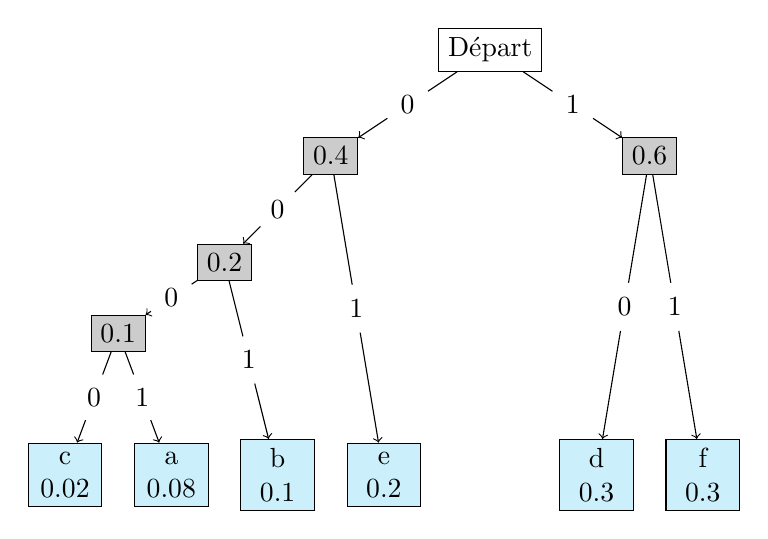
\begin{tikzpicture}[scale=0.9]
		\tikzstyle{etiquette}=[midway, circle ,fill=white]
		\node[draw] (D) at (0,0){Départ};	
		\node[draw, fill=black!20] (1) at (2.25,-1.5){0.6};
		\node[draw, fill=black!20] (0) at (-2.25,-1.5){0.4};
		\node[draw, text width=0.7cm, text centered, fill = cyan!20] (11) at (3,-6){f \\ 0.3};
		\node[draw, text width=0.7cm, text centered, fill = cyan!20] (10) at (1.5,-6){d \\ 0.3};
		\node[draw, text width=0.7cm, text centered, fill = cyan!20] (01) at (-1.5,-6){e \\ 0.2};
		\node[draw, fill=black!20] (00) at (-3.75,-3){0.2};
		\node[draw, text width=0.7cm, text centered, fill = cyan!20] (001) at (-3,-6){b \\ 0.1};
		\node[draw, fill=black!20] (000) at (-5.25,-4){0.1};
		\node[draw, text width=0.7cm, text centered, fill = cyan!20] (0001) at (-4.5,-6){a \\ 0.08};
		\node[draw, text width=0.7cm, text centered, fill = cyan!20] (0000) at (-6,-6){c \\ 0.02};

		\draw[->] (D) -- (0)node[etiquette]{0};
		\draw[->] (D) -- (1)node[etiquette]{1};
		\draw[->] (0) -- (00)node[etiquette]{0};
		\draw[->] (0) -- (01)node[etiquette]{1};
		\draw[->] (1) -- (10)node[etiquette]{0};
		\draw[->] (1) -- (11)node[etiquette]{1};
		\draw[->] (00) -- (000)node[etiquette]{0};
		\draw[->] (00) -- (001)node[etiquette]{1};
		\draw[->] (000) -- (0000)node[etiquette]{0};
		\draw[->] (000) -- (0001)node[etiquette]{1};
	\end{tikzpicture}\\
\end{center}
\setstretch{1.6}
Nous n'avons donc qu'à lire les positions afin de trouver le code associé :
\begin{tabular}{r|c|c|c|c|c|c}
	Symbole de source & a & b & c & d & e & f\\
		\hline
	Probabilité& 0.08 & 0.1 & 0.02 & 0.3 & 0.2 & 0.3\\
		\hline
	Code de Huffman& 0001 & 001 & 0000 & 10 & 10 & 11
\end{tabular}\\
\\
La longueur moyenne de ce code de Huffman est \\
$0.08\cdot 4 + 0.1 \cdot 3 + 0.02 \cdot 4 + 0.3 \cdot 2 + 0.2 \cdot 2 + 0.3 \cdot 2 =$ \fbox{$2.3 = L(\Gamma_H)$}\\
La longueur moyenne du code de Shannon-Fano est \\
$4\cdot 0.08 + 4\cdot 0.1 + 6\cdot 0.02 + 2\cdot 0.	3 + 3\cdot 0.2 + 2\cdot 0.3 =$ \fbox{$2.64 = L(\Gamma_{SF})$}\\
L'entropie de la source S, selon la méthode vue en cours, est\\
$0.08\cdot\log_2\left(\frac{1}{0.08}\right) + 0.1\cdot\log_2\left(\frac{1}{0.1}\right) + 0.02\cdot\log_2\left(\frac{1}{0.02}\right) + 0.3\cdot\log_2\left(\frac{1}{0.3}\right) + 0.2\cdot\log_2\left(\frac{1}{0.2}\right) + 0.3\cdot\log_2\left(\frac{1}{0.3}\right) =$ \fbox{$2.24 = H(S)$}\\
Ainsi, l'entropie est bien la plus petite valeur, et le code de Huffman est bien optimal (en tout cas par rapport au code de Shannon-Fano).\\
\\
La seconde inégalité de l'entropie est 
\begin{equation*}
	\frac{H(S)}{\log_2(D)} \leq L(\Gamma_{SF}) < \frac{H(S)}{\log_2(D)} +1
\end{equation*}
et elle est bien respectée pour le code de Shannon-Fano car
\begin{align*}
	2.24 \leq 2.64 < 3.24 = 2.24 +1\\
\end{align*}
de même que pour le code de Huffman (qui est optimal, donc meilleur ou égal à Shannon-Fano), car
\begin{equation*}
	2.24 \leq 2.3 < 3.24
\end{equation*}
\newpage
\item \underline{Premier arbre de Huffman $(H_1)$}
\begin{center}
		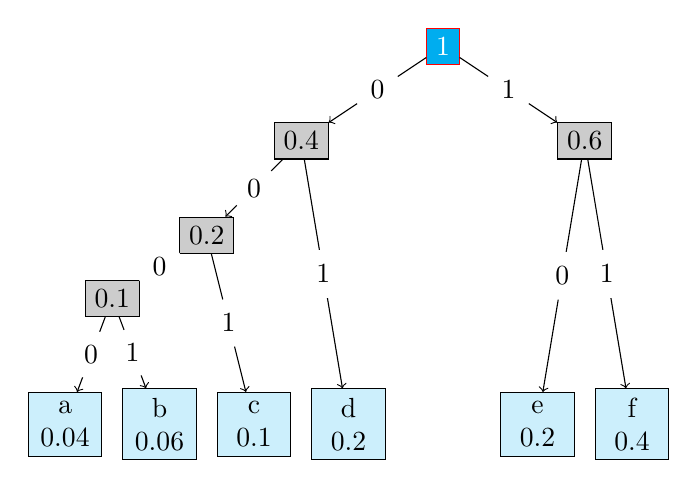
\begin{tikzpicture}[scale=0.8]
		\tikzstyle{etiquette}=[midway, circle ,fill=white]
		\node[draw, red, fill=cyan, text=white] (D) at (0,0){1};	
		\node[draw, fill=black!20] (1) at (2.25,-1.5){0.6};
		\node[draw, fill=black!20] (0) at (-2.25,-1.5){0.4};
		\node[draw, text width=0.7cm, text centered, fill = cyan!20] (11) at (3,-6){f \\ 0.4};
		\node[draw, text width=0.7cm, text centered, fill = cyan!20] (10) at (1.5,-6){e \\ 0.2};
		\node[draw, text width=0.7cm, text centered, fill = cyan!20] (01) at (-1.5,-6){d \\ 0.2};
		\node[draw, fill=black!20] (00) at (-3.75,-3){0.2};
		\node[draw, text width=0.7cm, text centered, fill = cyan!20] (001) at (-3,-6){c \\ 0.1};
		\node[draw, fill=black!20] (000) at (-5.25,-4){0.1};
		\node[draw, text width=0.7cm, text centered, fill = cyan!20] (0001) at (-4.5,-6){b \\ 0.06};
		\node[draw, text width=0.7cm, text centered, fill = cyan!20] (0000) at (-6,-6){a \\ 0.04};

		\draw[->] (D) -- (0)node[etiquette]{0};
		\draw[->] (D) -- (1)node[etiquette]{1};
		\draw[->] (0) -- (00)node[etiquette]{0};
		\draw[->] (0) -- (01)node[etiquette]{1};
		\draw[->] (1) -- (10)node[etiquette]{0};
		\draw[->] (1) -- (11)node[etiquette]{1};
		\draw[->] (00) -- (000)node[etiquette]{0};
		\draw[->] (00) -- (001)node[etiquette]{1};
		\draw[->] (000) -- (0000)node[etiquette]{0};
		\draw[->] (000) -- (0001)node[etiquette]{1};
	\end{tikzpicture}\\
\end{center}
Avec le code associé \\
\begin{tabular}{r|c|c|c|c|c|c}
Symbole de source & a & b & c & d & e & f\\
\hline
Probabilité& 0.04 & 0.06 & 0.1 & 0.2 & 0.2 & 0.4\\
\hline
$\Gamma_{H_1}$ & 0000 & 0001 & 001 & 01 & 10 & 11 
\end{tabular}\\
\\
\underline{Second arbre de Huffman $(H_2)$:}

\begin{center}
	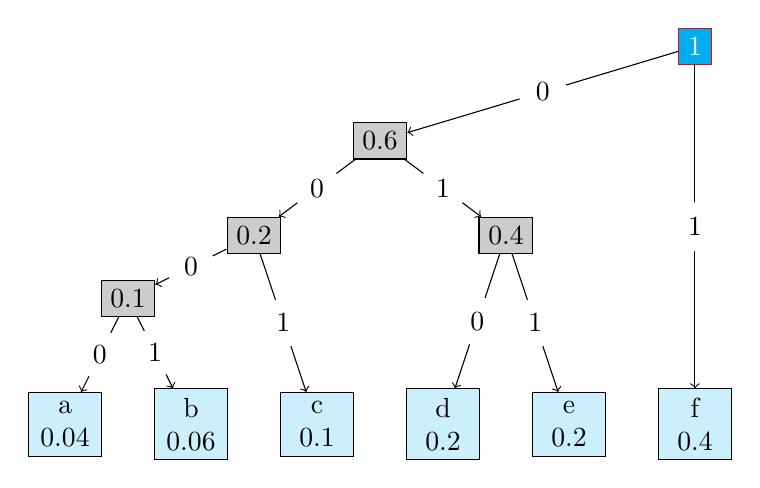
\begin{tikzpicture}[scale=0.8]
		\tikzstyle{etiquette}=[midway, circle ,fill=white]
		\node[draw, red, fill = cyan, text=white] (D) at (0,0){1};	
		\node[draw, fill=black!20] (0) at (-5,-1.5){0.6};
		\node[draw, text width=0.7cm, text centered, fill = cyan!20] (1) at (0,-6){f \\ 0.4};
		\node[draw, fill=black!20] (01) at (-3, -3){0.4};
		\node[draw, text width=0.7cm, text centered, fill = cyan!20] (011) at (-2,-6){e \\ 0.2};
		\node[draw, text width=0.7cm, text centered, fill = cyan!20] (010) at (-4,-6){d \\ 0.2};
		\node[draw, fill=black!20] (00) at (-7,-3){0.2};
		\node[draw, text width=0.7cm, text centered, fill = cyan!20] (001) at (-6,-6){c \\ 0.1};
		\node[draw, fill=black!20] (000) at (-9,-4){0.1};
		\node[draw, text width=0.7cm, text centered, fill = cyan!20] (0001) at (-8,-6){b \\ 0.06};
		\node[draw, text width=0.7cm, text centered, fill = cyan!20] (0000) at (-10,-6){a \\ 0.04};

		\draw[->] (D) -- (0)node[etiquette]{0};
		\draw[->] (D) -- (1)node[etiquette]{1};
		\draw[->] (0) -- (00)node[etiquette]{0};
		\draw[->] (0) -- (01)node[etiquette]{1};
		\draw[->] (01) -- (010)node[etiquette]{0};
		\draw[->] (01) -- (011)node[etiquette]{1};
		\draw[->] (00) -- (000)node[etiquette]{0};
		\draw[->] (00) -- (001)node[etiquette]{1};
		\draw[->] (000) -- (0000)node[etiquette]{0};
		\draw[->] (000) -- (0001)node[etiquette]{1};
	\end{tikzpicture}\\
\end{center}
Avec le code associé \\
\begin{tabular}{r|c|c|c|c|c|c}
Symbole de source & a & b & c & d & e & f\\
\hline
Probabilité& 0.04 & 0.06 & 0.1 & 0.2 & 0.2 & 0.4\\
\hline
$\Gamma_{H_2}$& 0000 & 0001 & 001 & 010 & 011 & 1 
\end{tabular}\\
\\
\\
$L(\Gamma_{H_1}) = 2\cdot0.4 + 2\cdot0.2 + 2\cdot 0.2 + 3\cdot 0.1 + 4\cdot 0.06 + 4\cdot 0.04 = 2.3$\\
$L(\Gamma_{H_2}) = 1\cdot0.4 + 3\cdot0.2 + 3\cdot 0.2 + 3\cdot 0.1 + 4\cdot 0.06 + 4\cdot 0.04 = 2.3$
\item Le théorème 3.4 du code de Huffman nous dit que \\
\textbf{[...]pour tout autre code binaire à décodage unique $\Gamma$ on a \\
$L(\Gamma_H) \leq L(\Gamma)$}\\
\\
Ce qui signifie que \\
$L(\Gamma_{H_1}) \leq L(\Gamma)$\\
mais aussi que \\
$L(\Gamma_{H_2}) \leq L(\Gamma)$\\
Donc que $(\Gamma_{H_2}) \leq (\Gamma_{H_1}) \leq (\Gamma_{H_2}) \leq (\Gamma)$\\
ce qui implique que $(\Gamma_{H_2}) = (\Gamma_{H_1})$	
\end{enumerate}
\evid{Problème 3.2}
\begin{enumerate}
	\item Nous pouvons utiliser la même formule qu'à l'exercice 3.1.1 ($\lceil\log_2\left(\frac{1}{p_i}\right)\rceil$)\\
	Cela nous donne les longueurs suivantes\\
	\begin{tabular}{r|c|c|c|c|c|c}
		Symbole de source & a & b & c & d & e & f\\
			\hline 
		Probabilité & $\frac{1}{16}$ & $\frac{1}{16}$ & $\frac{1}{8}$ & $\frac{1}{4}$ & $\frac{1}{4}$ & $\frac{1}{4}$\\
			\hline
		Longueur non-arrondie & 4 & 4 & 3 & 2 & 2  & 2\\
			\hline
		\textcolor{red}{Longueur arrondie} & \textcolor{red}{4} & \textcolor{red}{4} &\textcolor{red}{3} & \textcolor{red}{2} & \textcolor{red}{2} & \textcolor{red}{2}
	\end{tabular}\\
	Pour une longueur moyenne \\
	$L(\Gamma_{SF}) = \frac{4}{16} + \frac{4}{16} + \frac{3}{8} + \frac{2}{4} + \frac{2}{4} + \frac{2}{4} =$ \fbox{$2.375 = L(\Gamma_{SF})$}\\
	L'arbre de Huffman associé au code S est :\\
	\begin{center}
		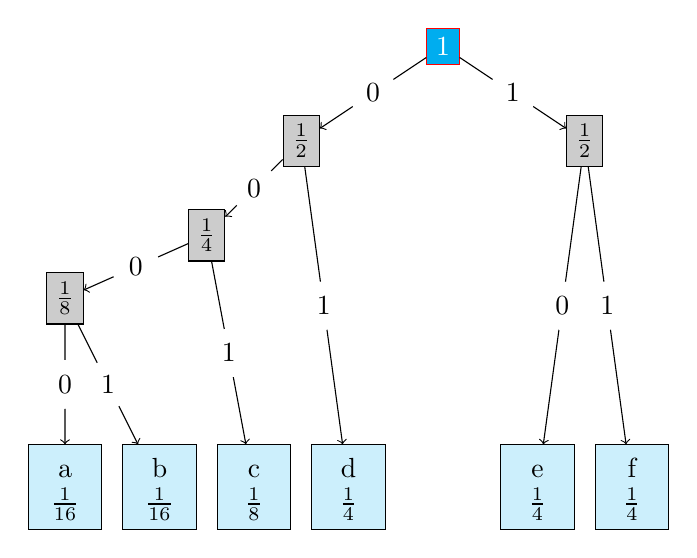
\begin{tikzpicture}[scale=0.8]
			\tikzstyle{etiquette}=[midway, circle ,fill=white]
	
			\node[draw, red, fill=cyan, text=white] (D) at (0,0){1};	
			\node[draw, fill=black!20] (1) at (2.25,-1.5){$\frac{1}{2}$};
			\node[draw, fill=black!20] (0) at (-2.25,-1.5){$\frac{1}{2}$};
			\node[draw, text width=0.7cm, text height  =0.3cm,text centered, fill = cyan!20] (11) at (3,-7){f \\ $\frac{1}{4}$};
			\node[draw, text width=0.7cm, text height  =0.3cm,text centered, fill = cyan!20] (10) at (1.5,-7){e \\ $\frac{1}{4}$};
			\node[draw, text width=0.7cm, text height  =0.3cm,text centered, fill = cyan!20] (01) at (-1.5,-7){d \\ $\frac{1}{4}$};
			\node[draw, fill=black!20] (00) at (-3.75,-3){$\frac{1}{4}$};
			\node[draw, text width=0.7cm, text height  =0.3cm,text centered, fill = cyan!20] (001) at (-3,-7){c \\ $\frac{1}{8}$};
			\node[draw, fill=black!20] (000) at (-6,-4){$\frac{1}{8}$};
			\node[draw, text width=0.7cm, text height  =0.3cm, text centered, fill = cyan!20] (0001) at (-4.5,-7){b \\ $\frac{1}{16}$};
			\node[draw, text width=0.7cm, text height  =0.3cm, text centered, fill = cyan!20] (0000) at (-6,-7){a \\ $\frac{1}{16}$};

			\draw[->] (D) -- (0)node[etiquette]{0};
			\draw[->] (D) -- (1)node[etiquette]{1};
			\draw[->] (0) -- (00)node[etiquette]{0};
			\draw[->] (0) -- (01)node[etiquette]{1};
			\draw[->] (1) -- (10)node[etiquette]{0};
			\draw[->] (1) -- (11)node[etiquette]{1};
			\draw[->] (00) -- (000)node[etiquette]{0};
			\draw[->] (00) -- (001)node[etiquette]{1};
			\draw[->] (000) -- (0000)node[etiquette]{0};	
			\draw[->] (000) -- (0001)node[etiquette]{1};
		\end{tikzpicture}\\
	\end{center}
	Avec le code qui en découle : \\
	\begin{tabular}{r|c|c|c|c|c|c}
		Symbole de source & a & b & c & d & e & f\\
			\hline
		Probabilité & $\frac{1}{16}$ & $\frac{1}{16}$ & $\frac{1}{8}$ & $\frac{1}{4}$ & $\frac{1}{4}$ & $\frac{1}{4}$\\
			\hline
		$\Gamma_{H}$ & 0000 & 0001 & 001 & 01 & 10 & 11 
	\end{tabular}\\
	La longueur moyenne de ce code est :\\
	$\frac{4}{16} + \frac{4}{16} + \frac{3}{8} + \frac{2}{4}+ \frac{2}{4}+ \frac{2}{4} = $ \fbox{$2.375 = L(\Gamma_H)$}
	\\
	L'entropie de la source S est \\
	$2\cdot\frac{1}{16}\log_2(16) + \frac{1}{8}\log_2(8) + 3\cdot\frac{1}{4}\log_2(4) = $ \fbox{$2.375 = H(S)$}\\
	\\
	Il est alors amusant de constater (nous le prouverons à la question suivante) que les 3 longueurs sont exactement les mêmes.
	\item 
		\begin{enumerate}[label=(\alph*)]
			\item Ce qui fait varier la  longueur des mots de code de Shannon par rapport à l'entropie, c'est l'arrondi vers le haut. En effet, là où l'entropie multiplie la probabilité d'apparition par le log de l'inverse de cette probabilité ($\sum p(s)\log_2(\frac{1}{p(s)})$), la longueurs selon Shannon multiplie la probabilité d'apparition par \underline{l'arrondi vers le haut} de ce même logarithme ; la longueur du mot de code est $\lceil\log_2(\frac{1}{p(s)})\rceil$, et pour trouver la longueur moyenne nous multiplions les mots de code par leur probabilité d'apparition, ce qui nous donne $\sum p(s)\lceil\log_2(\frac{1}{p(s)})\rceil$. Mais lorsque les $p(s)$ sont des puissances de 2, alors $\lceil\log_2(\frac{1}{p(s)})\rceil = \log_2(\frac{1}{p(s)})$ (car $\log_2(2^n) = n$). La longueurs des mots de Shannon ont alors la même longueur (car même formule) que l'entropie.
			\item Comme nous l'avons dit avant, $L(\Gamma_{SF}) = \sum p(s)\lceil\log_2(\frac{1}{p(s)})\rceil = \sum p(s)\log_2(\frac{1}{p(s)}) = H(S)$ quand et seulement quand tous les $p(s)$ sont des puissances de 2, car l'arrondi n'a plus lieu (le $\log_2$ étant alors déjà entier). Ainsi, lorsque $L(\Gamma_{SF})$ devient plus grand que l'entropie, cela signifie qu'une longueur a été arrondie vers le haut (selon la définition), et donc qu'un des $p(s)$ n'est plus une puissance de 2.
		\end{enumerate}
\end{enumerate}
\evid{Problème 3.3}
\begin{enumerate}
	\item \begin{tabular}{c|c}
	A & B\\
	\hline
	$\frac{3}{4}$ & $\frac{1}{4}$
	\end{tabular}. L'entropie est donc $\frac{3}{4}\log_2\left(\frac{4}{3}\right) + \frac{1}{4}\log_2(4) = $ \fbox{$0.811 = H(S_0)$}
	\item $H(S_1|S_0) = H(S_1|S_0 = A)p_{S_0}(A) + H(S_1|S_0 = B)p_{S_0}(B)$\\
		$H(S_1|S_0 = A) = \frac{1}{2}\log_2(2) + \frac{1}{2}\log_2(2) = 2\frac{1}{2}\log_2(2) = 1$\\ \big(car 2 issues possibles (P/F) avec chacun probabilité 1/2\big)\\
		$H(S_1|S_0 = B) = 1\log_2(1) = 0$\\ \big(car seulement F possible, avec probabilité 1\big)\\	
		$p_{S_0}(A) = \frac{3}{4}, p_{S_0}(B) = \frac{1}{4} \to H(S_1|S_0) = \frac{3}{4}\cdot 1 + \frac{1}{4}\cdot 0 = $ \fbox{$\frac{3}{4} = H(S_1|S_0)$}\\
		\\
		$H(S_2|S_0) = H(S_2|S_0 = A)p_{S_0}(A) + H(S_2|S_0 = B)p_{S_0}(B)$\\
		$H(S_2|S_0 = A) = \frac{1}{2}\log_2(2) + \frac{1}{2}\log_2(2) = 2\frac{1}{2}\log_2(2) = 1$\\
		$H(S_2|S_0 = B) = 1\log_2(1) = 0$\\
		(mêmes justifications que pour $H(S_1|S_0)$)\\
		$p_{S_0}(A) = \frac{3}{4}, p_{S_0}(B) = \frac{1}{4} \to H(S_2|S_0) = \frac{3}{4}\cdot 1 + 	\frac{1}{4}\cdot 0 = $ \fbox{$\frac{3}{4} = H(S_2|S_0)$}\\
		\\
		$H(S|S_0) = H(S|S_0=A)p_{S_0}(A) + H(S|S_0=B)p_{S_0}(B)$\\
		$p_{S_0}(A) = \frac{3}{4}, \ p_{S_0}(B) = \frac{1}{4}$\\
		$H(S|S_0=B) = 1\log_2(1) = 0$\\
		(car seulement FF possible, avec probabilité 1)\\
		$H(S|S_0 =A) = 4\cdot\frac{1}{4}\log_2(4) = 2$\\
		(car 4 issues possibles PF, FP, FF, PP, chacun avec probabilité $\frac{1}{2}\cdot\frac{1}{2} = \frac{1}{4}$)
		$\to H(S|S_0) = \frac{3}{4}\cdot2+\frac{1}{4}\cdot0 =$ \fbox{$\frac{3}{2} = H(S|S_0)$} 
		\\
		Nous remarquons - à notre immense étonnement - que $H(S_2|S_0) = H(S_1|S_0)$. En effet, l'ordre des tirages n'a pas d'importance, une fois que l'on connaît $S_0$. Pile arrivera avec la même probabilité que face ($\frac{1}{2}$) si la pièce A est prise, et Face arrivera forcément si B est prise, les probabilités ne changent pas $\to$ \fbox{$H(S_2|S_0) = \frac{3}{4} = H(S_1|S_0)$}
	\item Pour $S_1$ nous avons la densité de probabilité suivante :
		\begin{tabular}{r|l}
			Outcome possible & Probabilité\\
				\hline
			P & 3/8\\
			F & 5/8
		\end{tabular}\\
		En effet, $\begin{array}{l}
		p(P) = p(AP) + P(BP) = \frac{3}{8} + 0\\
		p(F) = p(AF) + P(BF) = \frac{3}{8} +  \frac{1}{4} = \frac{5}{8}
		\end{array}$
		
		 $H(S_1) = \frac{3}{8}\log_2(\frac{8}{3}) + \frac{5}{8}\log_2(\frac{8}{5}) = $ \fbox{$0.954 = H(S_1)$}\\
		\\
		Pour $S_2$, la densité de probabilité est 
		\begin{tabular}{r|l}
			Outcome possible & Probabilité\\
				\hline
			P & 3/8\\
			F & 5/8\\
		\end{tabular}
		(Mêmes explications que pour $S_1$). La densité de probabilité étant la même, l'entropie est donc la même aussi $\to$ \fbox{$0.954 = H(S_2)$}\\
		Pour $S$ en revanche, la densité de probabilité change légèrement : 
		\begin{tabular}{r|l}
			Outcome possible & Probabilité\\
				\hline
			PP & 3/16\\
			PF & 3/16\\
			FP & 3/16\\
			FF & 7/16\\
		\end{tabular}\\
		Car $\left\{\begin{array}{l}
		p(PP) = p(APP) + p(BPP) = \frac{3}{16} + 0= \frac{3}{16}\\
		p(PF) = p(APP) + p(BPF) = \frac{3}{16} + 0= \frac{3}{16}\\
		p(FP) = p(AFP) + p(BFP) = \frac{3}{16} + 0 = \frac{3}{16}\\
		p(PP) = p(APP) + p(BPP) = \frac{3}{16} + \frac{1}{4}= \frac{7}{16}\\
		\end{array}\right\}$\\
		Donc $H(S) = 3\cdot\frac{3}{16}\log_2(\frac{16}{3}) + \frac{7}{16}\log_2(\frac{16}{7}) = $ \fbox{$1.88 = H(S)$}. 
		 $H(S_1|S_0) = \frac{3}{4} \leq 0.954	=	H(S_1)$ et $H(S_1,S_2|S_0) = \frac{3}{2} \leq 1.88 = H(S)$. Cela semble correcte, car ces inégalités répondent au théorème 4.2(Conditionner réduit l'entropie). En effet, savoir $S_0$ nous apporte une information supplémentaire (caractérisée par la différence entre les deux termes d'une inégalité) ; ayant plus d'information, l'entropie s'en trouve donc réduite.
	\item $p_{S_2|S_1}(s_2|s_1)$ = \enquote{probabilité que $S_2 = s_2$ sachant que $S_1 = s_1$} = $\frac{p(s_1,s_2)}{p(s_1)}$ Nous pouvons donc analyser les cas un par un\footnote{c.f. partie 3 pour les probabilités} :
		\begin{itemize}
			\item $p_{S_2|S_1}(P|P) = \frac{1}{2}$ Une fois que le premier tirage est fait et que pile est sorti, on sait que la pièce est A. La probabilité d'avoir pile est donc de $\frac{1}{2}$
			\item $p_{S_2|S_1}(F|P) = \frac{1}{2}$, pour la même raison qu'au-dessus. Pile est sorti, donc nous savons que la pièce est A, donc une chance sur deux d'avoir pile, et une demi pour face.
			\item $p_{S_2|S_1}(P|F) = \frac{p_{S_1,S_2}(FP)}{p_{S_1}(F)} = \frac{\frac{3}{16}}{\frac{5}{8}} = \frac{3}{10}$
			\item $p_{S_2|S_1}(F|F) = \frac{p_{S_1,S_2}(FF)}{p_{S_1}(F)} = \frac{\frac{7}{10}}{\frac{5}{8}} = \frac{7}{10}$
		\end{itemize}
	\item $H(S_2|S_1) = \somme{}{s_1\in A_1} H(S_2|S_1=s_1)p_{S_1}(s_1)$\\
	$\to = H(S_2|S_1 =P)p_{S_1}(P) + H(S_2|S_1 = F)p_{S_1}(F)$\\
	$p_{S_1}(P) = \frac{3}{8},\ p_{S_1}(F) =\frac{5}{8}$ \\
	$H(S_2|S_1=P) = 2\cdot\frac{1}{2}\log_2(2) = 1$\\
	$H(S_2|S_1=F) = \frac{3}{10}\log_2(\frac{10}{3}) + \frac{7}{10}\log_2(\frac{10}{7}) \simeq 0.8813$\\
	$\to H(S_2|S_1) = \frac{5}{8}\cdot 0.8813 + \frac{3}{8}\cdot 1 \simeq$ \fbox{0.926 = $H(S_2|S_1)$}\\
	Cette entropie est plus faible que celle de $S_2$ (ce qui répond au théorème 4.2), car une fois que l'on sait $S_1$, nous sommes dirigés vers une solution : Si face apparaît, nous serons tentés de proposer face au tirage suivant. Cette tentation est caractérisée par une entropie inférieure.
	\item La règle de l'enchaînement pour l'entropie semble être :\\
	$H(S_2|S_1) = H(S_2,S_1)-H(S_1) = H(S)-H(S_1) = 1.88-0.954 = 0.926$. La valeur de cette entropie est donc vérifiée.
	\item La densité de probabilité est (dans l'ordre $S_0, S_1, S_2$)
		\begin{tabular}{r|l}
			Outcome possible & probabilité\\
				\hline
			APP & 3/16\\
			APF & 3/16\\
			AFP & 3/16\\
			AFF & 3/16\\
			BPP & 0\\
			BPF & 0\\
			BFP & 0\\
			BFF & 1/4	
		\end{tabular}\\
		Donc l'entropie de cette source est : $4\cdot\frac{3}{16}\log_2(\frac{16}{3}) + \frac{1}{4}\log_2(4) =$ \fbox{$2.311 = H(S_0,S_1,S_2)$}\\
	\item $H(S_2|S_1,S_0) = H(S_2|S_1,S_0 = PA)\cdot p_{S_1,S_0}(PA) + 
							H(S_2|S_1,S_0 = FA)\cdot p_{S_1,S_0}(FA) +
							H(S_2|S_1,S_0 = PB)\cdot p_{S_1,S_0}(PB) +
							H(S_2|S_1,S_0 = FB)\cdot p_{S_1,S_0}(FB)$\\
		\begin{tabular}{r|l}
		Outcome & proba\\
		\hline
		$p_{S_1,S_0}(FB)$ & $\frac{1}{4}$\\
		$p_{S_1,S_0}(PB)$ & $0$\\
		$p_{S_1,S_0}(FA)$ & $\frac{3}{8}$\\
		$p_{S_1,S_0}(PA)$ & $\frac{3}{8}$
		\end{tabular}\\
		$H(S_2|S_1,S_0 = PA) = H(S_2|S_1,S_0 = FA)= 2\cdot\frac{1}{2}\log_2(2) = 1\\
		H(S_2|S_1,S_0 = PA) = 0$ (cas impossible)\\
		$H(S_2|S_1,S_0 = FB) = 1\log_2(1) = 0$ (source déterministe).\\
		$\to H(S_2|S_1,S_0) = 2\cdot\frac{3}{8}\cdot 1 =$ \fbox{$\frac{3}{4} = H(S_2|S_1,S_0)$}.\\
		Nous voyons que $H(S_2|S_1,S_0) = H(S_2|S_0)$. En effet, savoir $S_1$ en plus ne nous donnera aucune information en plus ; Si la pièce est A, alors Pile et Face arriveront toujours avec la même probabilité (jets indépendants), et si la pièce est B alors Face sortira tout le temps $\to$ connaître le premier tirage (si l'on sait quelle pièce est utilisée) ne nous fournit aucune information supplémentaire sur $S_2$.
		\item $H(S_0|S_1,S_2) = H(S_0|S) = H(S_0,S) - H(S) = H(S_0,S_1,S_2)-H(S_1,S_2) = 2.311 - 1.88 = $\fbox{$0.431 =H(S_0|S_1,S_2)$}
	
\end{enumerate}
\end{document}